% Options for packages loaded elsewhere
\PassOptionsToPackage{unicode}{hyperref}
\PassOptionsToPackage{hyphens}{url}
%
\documentclass[
]{article}
\usepackage{lmodern}
\usepackage{amssymb,amsmath}
\usepackage{ifxetex,ifluatex}
\ifnum 0\ifxetex 1\fi\ifluatex 1\fi=0 % if pdftex
  \usepackage[T1]{fontenc}
  \usepackage[utf8]{inputenc}
  \usepackage{textcomp} % provide euro and other symbols
\else % if luatex or xetex
  \usepackage{unicode-math}
  \defaultfontfeatures{Scale=MatchLowercase}
  \defaultfontfeatures[\rmfamily]{Ligatures=TeX,Scale=1}
\fi
% Use upquote if available, for straight quotes in verbatim environments
\IfFileExists{upquote.sty}{\usepackage{upquote}}{}
\IfFileExists{microtype.sty}{% use microtype if available
  \usepackage[]{microtype}
  \UseMicrotypeSet[protrusion]{basicmath} % disable protrusion for tt fonts
}{}
\makeatletter
\@ifundefined{KOMAClassName}{% if non-KOMA class
  \IfFileExists{parskip.sty}{%
    \usepackage{parskip}
  }{% else
    \setlength{\parindent}{0pt}
    \setlength{\parskip}{6pt plus 2pt minus 1pt}}
}{% if KOMA class
  \KOMAoptions{parskip=half}}
\makeatother
\usepackage{xcolor}
\IfFileExists{xurl.sty}{\usepackage{xurl}}{} % add URL line breaks if available
\IfFileExists{bookmark.sty}{\usepackage{bookmark}}{\usepackage{hyperref}}
\hypersetup{
  hidelinks,
  pdfcreator={LaTeX via pandoc}}
\urlstyle{same} % disable monospaced font for URLs
\usepackage[margin=1in]{geometry}
\usepackage{color}
\usepackage{fancyvrb}
\newcommand{\VerbBar}{|}
\newcommand{\VERB}{\Verb[commandchars=\\\{\}]}
\DefineVerbatimEnvironment{Highlighting}{Verbatim}{commandchars=\\\{\}}
% Add ',fontsize=\small' for more characters per line
\usepackage{framed}
\definecolor{shadecolor}{RGB}{248,248,248}
\newenvironment{Shaded}{\begin{snugshade}}{\end{snugshade}}
\newcommand{\AlertTok}[1]{\textcolor[rgb]{0.94,0.16,0.16}{#1}}
\newcommand{\AnnotationTok}[1]{\textcolor[rgb]{0.56,0.35,0.01}{\textbf{\textit{#1}}}}
\newcommand{\AttributeTok}[1]{\textcolor[rgb]{0.77,0.63,0.00}{#1}}
\newcommand{\BaseNTok}[1]{\textcolor[rgb]{0.00,0.00,0.81}{#1}}
\newcommand{\BuiltInTok}[1]{#1}
\newcommand{\CharTok}[1]{\textcolor[rgb]{0.31,0.60,0.02}{#1}}
\newcommand{\CommentTok}[1]{\textcolor[rgb]{0.56,0.35,0.01}{\textit{#1}}}
\newcommand{\CommentVarTok}[1]{\textcolor[rgb]{0.56,0.35,0.01}{\textbf{\textit{#1}}}}
\newcommand{\ConstantTok}[1]{\textcolor[rgb]{0.00,0.00,0.00}{#1}}
\newcommand{\ControlFlowTok}[1]{\textcolor[rgb]{0.13,0.29,0.53}{\textbf{#1}}}
\newcommand{\DataTypeTok}[1]{\textcolor[rgb]{0.13,0.29,0.53}{#1}}
\newcommand{\DecValTok}[1]{\textcolor[rgb]{0.00,0.00,0.81}{#1}}
\newcommand{\DocumentationTok}[1]{\textcolor[rgb]{0.56,0.35,0.01}{\textbf{\textit{#1}}}}
\newcommand{\ErrorTok}[1]{\textcolor[rgb]{0.64,0.00,0.00}{\textbf{#1}}}
\newcommand{\ExtensionTok}[1]{#1}
\newcommand{\FloatTok}[1]{\textcolor[rgb]{0.00,0.00,0.81}{#1}}
\newcommand{\FunctionTok}[1]{\textcolor[rgb]{0.00,0.00,0.00}{#1}}
\newcommand{\ImportTok}[1]{#1}
\newcommand{\InformationTok}[1]{\textcolor[rgb]{0.56,0.35,0.01}{\textbf{\textit{#1}}}}
\newcommand{\KeywordTok}[1]{\textcolor[rgb]{0.13,0.29,0.53}{\textbf{#1}}}
\newcommand{\NormalTok}[1]{#1}
\newcommand{\OperatorTok}[1]{\textcolor[rgb]{0.81,0.36,0.00}{\textbf{#1}}}
\newcommand{\OtherTok}[1]{\textcolor[rgb]{0.56,0.35,0.01}{#1}}
\newcommand{\PreprocessorTok}[1]{\textcolor[rgb]{0.56,0.35,0.01}{\textit{#1}}}
\newcommand{\RegionMarkerTok}[1]{#1}
\newcommand{\SpecialCharTok}[1]{\textcolor[rgb]{0.00,0.00,0.00}{#1}}
\newcommand{\SpecialStringTok}[1]{\textcolor[rgb]{0.31,0.60,0.02}{#1}}
\newcommand{\StringTok}[1]{\textcolor[rgb]{0.31,0.60,0.02}{#1}}
\newcommand{\VariableTok}[1]{\textcolor[rgb]{0.00,0.00,0.00}{#1}}
\newcommand{\VerbatimStringTok}[1]{\textcolor[rgb]{0.31,0.60,0.02}{#1}}
\newcommand{\WarningTok}[1]{\textcolor[rgb]{0.56,0.35,0.01}{\textbf{\textit{#1}}}}
\usepackage{graphicx}
\makeatletter
\def\maxwidth{\ifdim\Gin@nat@width>\linewidth\linewidth\else\Gin@nat@width\fi}
\def\maxheight{\ifdim\Gin@nat@height>\textheight\textheight\else\Gin@nat@height\fi}
\makeatother
% Scale images if necessary, so that they will not overflow the page
% margins by default, and it is still possible to overwrite the defaults
% using explicit options in \includegraphics[width, height, ...]{}
\setkeys{Gin}{width=\maxwidth,height=\maxheight,keepaspectratio}
% Set default figure placement to htbp
\makeatletter
\def\fps@figure{htbp}
\makeatother
\setlength{\emergencystretch}{3em} % prevent overfull lines
\providecommand{\tightlist}{%
  \setlength{\itemsep}{0pt}\setlength{\parskip}{0pt}}
\setcounter{secnumdepth}{-\maxdimen} % remove section numbering

\author{}
\date{\vspace{-2.5em}}

\begin{document}

\hypertarget{moleculeexperiment}{%
\section{MoleculeExperiment}\label{moleculeexperiment}}

The R package MoleculeExperiment contains functions to create and work
with the MoleculeExperiment class. We introduce this class for analysing
molecule-based spatial transcriptomics data (xenium by 10x, cosmx SMI by
nanostring, and merscope by vizgen).

\hypertarget{contents}{%
\section{Contents}\label{contents}}

TODO Have hyperlinks here 1. Why the MoleculeExperiment class 2. The ME
object \ldots{}

\hypertarget{why-the-moleculeexperiment-class}{%
\section{Why the MoleculeExperiment
class?}\label{why-the-moleculeexperiment-class}}

\begin{enumerate}
\def\labelenumi{\arabic{enumi})}
\tightlist
\item
  Enable easy analysis of spatial transcriptomics data at the molecule
  level, rather than the cell level.
\item
  Standardisation of molecule-based ST data across vendors, to hopefully
  facilitate comparison of different data sources.
\end{enumerate}

\hypertarget{the-me-object}{%
\section{The ME object}\label{the-me-object}}

\hypertarget{constructing-an-me-object}{%
\subsection{Constructing an ME object}\label{constructing-an-me-object}}

\begin{Shaded}
\begin{Highlighting}[]
\CommentTok{\# load necessary libraries}
\KeywordTok{library}\NormalTok{(devtools)}
\end{Highlighting}
\end{Shaded}

\begin{verbatim}
## Loading required package: usethis
\end{verbatim}

\begin{Shaded}
\begin{Highlighting}[]
\KeywordTok{load\_all}\NormalTok{()}
\end{Highlighting}
\end{Shaded}

\begin{verbatim}
## i Loading SpatialUtils
\end{verbatim}

\begin{Shaded}
\begin{Highlighting}[]
\CommentTok{\#library(MoleculeExperiment)}
\KeywordTok{library}\NormalTok{(ggplot2)}
\end{Highlighting}
\end{Shaded}

\hypertarget{usecase-1}{%
\subsubsection{usecase 1}\label{usecase-1}}

We will demonstrate how to generate an ME object with toy data
representing a scenario where both the detected transcripts information
and the boundary information is read into R.

First we generate a toy transcripts data.frame:

\begin{Shaded}
\begin{Highlighting}[]
\CommentTok{\# molecules data.frame toy example}
\NormalTok{molecules\_df \textless{}{-}}\StringTok{ }\KeywordTok{data.frame}\NormalTok{(}
  \DataTypeTok{sample\_id =} \KeywordTok{rep}\NormalTok{(}\KeywordTok{c}\NormalTok{(}\StringTok{"sample1"}\NormalTok{, }\StringTok{"sample2"}\NormalTok{), }\DataTypeTok{times =} \KeywordTok{c}\NormalTok{(}\DecValTok{30}\NormalTok{, }\DecValTok{20}\NormalTok{)),}
  \DataTypeTok{feature\_name =} \KeywordTok{rep}\NormalTok{(}\KeywordTok{c}\NormalTok{(}\StringTok{"gene1"}\NormalTok{, }\StringTok{"gene2"}\NormalTok{), }\DataTypeTok{times =} \KeywordTok{c}\NormalTok{(}\DecValTok{20}\NormalTok{, }\DecValTok{30}\NormalTok{)),}
  \DataTypeTok{x\_location =} \KeywordTok{runif}\NormalTok{(}\DecValTok{50}\NormalTok{),}
  \DataTypeTok{y\_location =} \KeywordTok{runif}\NormalTok{(}\DecValTok{50}\NormalTok{)}
\NormalTok{  )}
\KeywordTok{head}\NormalTok{(molecules\_df)}
\end{Highlighting}
\end{Shaded}

\begin{verbatim}
##   sample_id feature_name x_location y_location
## 1   sample1        gene1 0.39662798  0.5046235
## 2   sample1        gene1 0.44778193  0.9488975
## 3   sample1        gene1 0.99068979  0.2600446
## 4   sample1        gene1 0.20336426  0.1255218
## 5   sample1        gene1 0.03030918  0.4976240
## 6   sample1        gene1 0.55542501  0.1471956
\end{verbatim}

Then we generate a toy boundaries data.frame:

\begin{Shaded}
\begin{Highlighting}[]
\CommentTok{\# boundaries data.frame toy example}
\NormalTok{boundaries\_df \textless{}{-}}\StringTok{ }\KeywordTok{data.frame}\NormalTok{(}
  \DataTypeTok{sample\_id =} \KeywordTok{rep}\NormalTok{(}\KeywordTok{c}\NormalTok{(}\StringTok{"sample1"}\NormalTok{, }\StringTok{"sample2"}\NormalTok{), }\DataTypeTok{times =} \KeywordTok{c}\NormalTok{(}\DecValTok{16}\NormalTok{, }\DecValTok{6}\NormalTok{)),}
  \DataTypeTok{cell\_id =} \KeywordTok{rep}\NormalTok{(}\KeywordTok{c}\NormalTok{(}\StringTok{"cell1"}\NormalTok{, }\StringTok{"cell2"}\NormalTok{, }\StringTok{"cell3"}\NormalTok{, }\StringTok{"cell4"}\NormalTok{,}
                  \StringTok{"cell1"}\NormalTok{, }\StringTok{"cell2"}\NormalTok{),}
                \DataTypeTok{times =} \KeywordTok{c}\NormalTok{(}\DecValTok{4}\NormalTok{, }\DecValTok{4}\NormalTok{, }\DecValTok{4}\NormalTok{, }\DecValTok{4}\NormalTok{, }\DecValTok{3}\NormalTok{, }\DecValTok{3}\NormalTok{)),}
  \DataTypeTok{x\_location =} \KeywordTok{c}\NormalTok{(}\DecValTok{0}\NormalTok{, }\FloatTok{0.5}\NormalTok{, }\FloatTok{0.5}\NormalTok{, }\DecValTok{0}\NormalTok{,}
                 \FloatTok{0.5}\NormalTok{, }\DecValTok{1}\NormalTok{, }\DecValTok{1}\NormalTok{, }\FloatTok{0.5}\NormalTok{,}
                 \DecValTok{0}\NormalTok{, }\FloatTok{0.5}\NormalTok{, }\FloatTok{0.5}\NormalTok{, }\DecValTok{0}\NormalTok{,}
                 \FloatTok{0.5}\NormalTok{, }\DecValTok{1}\NormalTok{, }\DecValTok{1}\NormalTok{, }\FloatTok{0.5}\NormalTok{,}
                 \DecValTok{0}\NormalTok{, }\DecValTok{1}\NormalTok{, }\DecValTok{0}\NormalTok{,}
                 \DecValTok{0}\NormalTok{, }\DecValTok{1}\NormalTok{, }\DecValTok{1}\NormalTok{),}
  \DataTypeTok{y\_location =} \KeywordTok{c}\NormalTok{(}\DecValTok{0}\NormalTok{, }\DecValTok{0}\NormalTok{, }\FloatTok{0.5}\NormalTok{, }\FloatTok{0.5}\NormalTok{,}
                 \DecValTok{0}\NormalTok{, }\DecValTok{0}\NormalTok{, }\FloatTok{0.5}\NormalTok{, }\FloatTok{0.5}\NormalTok{,}
                 \FloatTok{0.5}\NormalTok{, }\FloatTok{0.5}\NormalTok{, }\DecValTok{1}\NormalTok{, }\DecValTok{1}\NormalTok{,}
                 \FloatTok{0.5}\NormalTok{, }\FloatTok{0.5}\NormalTok{, }\DecValTok{1}\NormalTok{, }\DecValTok{1}\NormalTok{,}
                 \DecValTok{0}\NormalTok{, }\DecValTok{1}\NormalTok{, }\DecValTok{1}\NormalTok{,}
                 \DecValTok{0}\NormalTok{, }\DecValTok{0}\NormalTok{, }\DecValTok{1}\NormalTok{)}
\NormalTok{)}
\KeywordTok{head}\NormalTok{(boundaries\_df)}
\end{Highlighting}
\end{Shaded}

\begin{verbatim}
##   sample_id cell_id x_location y_location
## 1   sample1   cell1        0.0        0.0
## 2   sample1   cell1        0.5        0.0
## 3   sample1   cell1        0.5        0.5
## 4   sample1   cell1        0.0        0.5
## 5   sample1   cell2        0.5        0.0
## 6   sample1   cell2        1.0        0.0
\end{verbatim}

To generate an ME object, the next step is to standardise these lists to
the MoleculeExperiment list. This consists of a list of lists,
ultimately ending in a tibble. This data structure was used to store
disk space, as data in a list enables us to avoid redundantly storing
gene names or sample IDs for the millions of transcripts. In the case of
the molecules information, we would like to store the information in a
list of lists with the following structure: ``sample ID'' \textgreater{}
``feature name'' \textgreater{} tibble with X and Y locations (and other
additional columns of interest). Additionally, one might like to filter
the transcripts and store them in the same object, in which case one can
also have this structure: ``filtered'' \textgreater{} ``sample ID''
\textgreater{} ``feature name'' \textgreater{} tibble.

\begin{Shaded}
\begin{Highlighting}[]
\NormalTok{molecules\_ls \textless{}{-}}\StringTok{ }\KeywordTok{dataframeToMEList}\NormalTok{(molecules\_df,}
                                  \DataTypeTok{df\_type =} \StringTok{"transcripts"}\NormalTok{,}
                                  \DataTypeTok{assay\_name =} \StringTok{"raw"}\NormalTok{,}
                                  \DataTypeTok{sample\_col =} \StringTok{"sample\_id"}\NormalTok{,}
                                  \DataTypeTok{factor\_col =} \StringTok{"feature\_name"}\NormalTok{,}
                                  \DataTypeTok{x\_col =} \StringTok{"x\_location"}\NormalTok{,}
                                  \DataTypeTok{y\_col =} \StringTok{"y\_location"}\NormalTok{)}
\CommentTok{\# to avoid printing large nested list in the terminal, use str() and the}
\CommentTok{\# max.level argument}
\KeywordTok{str}\NormalTok{(molecules\_ls, }\DataTypeTok{max.level =} \DecValTok{3}\NormalTok{)}
\end{Highlighting}
\end{Shaded}

\begin{verbatim}
## List of 1
##  $ raw:List of 2
##   ..$ sample1:List of 2
##   .. ..$ gene1: tibble [20 x 2] (S3: tbl_df/tbl/data.frame)
##   .. ..$ gene2: tibble [10 x 2] (S3: tbl_df/tbl/data.frame)
##   ..$ sample2:List of 1
##   .. ..$ gene2: tibble [20 x 2] (S3: tbl_df/tbl/data.frame)
\end{verbatim}

For the boundaries slot, if the boundary information is for cells, the
structure would look like this: ``cells'' \textgreater{} ``sample ID''
\textgreater{} ``cell IDs'' \textgreater{} tibble with the vertex
coordinates defining the boundaries for each cell. If the boundary
information is for nuclei, the structure would be: ``nuclei''
\textgreater{} ``sample ID'' \textgreater{} ``cell ID'' \textgreater{}
tibble with the vertex coordinates defining the boundary information for
the nuclei.

\begin{Shaded}
\begin{Highlighting}[]
\NormalTok{boundaries\_ls \textless{}{-}}\StringTok{ }\KeywordTok{dataframeToMEList}\NormalTok{(boundaries\_df,}
                                   \DataTypeTok{df\_type =} \StringTok{"boundaries"}\NormalTok{,}
                                   \DataTypeTok{assay\_name =} \StringTok{"cells"}\NormalTok{,}
                                   \DataTypeTok{sample\_col =} \StringTok{"sample\_id"}\NormalTok{,}
                                   \DataTypeTok{factor\_col =} \StringTok{"cell\_id"}\NormalTok{,}
                                   \DataTypeTok{x\_col =} \StringTok{"x\_location"}\NormalTok{,}
                                   \DataTypeTok{y\_col =} \StringTok{"y\_location"}\NormalTok{)}
\KeywordTok{str}\NormalTok{(boundaries\_ls, }\DecValTok{3}\NormalTok{)}
\end{Highlighting}
\end{Shaded}

\begin{verbatim}
## List of 1
##  $ cells:List of 2
##   ..$ sample1:List of 4
##   .. ..$ cell1: tibble [4 x 2] (S3: tbl_df/tbl/data.frame)
##   .. ..$ cell2: tibble [4 x 2] (S3: tbl_df/tbl/data.frame)
##   .. ..$ cell3: tibble [4 x 2] (S3: tbl_df/tbl/data.frame)
##   .. ..$ cell4: tibble [4 x 2] (S3: tbl_df/tbl/data.frame)
##   ..$ sample2:List of 2
##   .. ..$ cell1: tibble [3 x 2] (S3: tbl_df/tbl/data.frame)
##   .. ..$ cell2: tibble [3 x 2] (S3: tbl_df/tbl/data.frame)
\end{verbatim}

Now that the transcript and boundary information is in a standardised
format, it can be used as input to generate an ME object.

\begin{Shaded}
\begin{Highlighting}[]
\CommentTok{\# use MoleculeExperiment object constructor}
\NormalTok{toy\_me \textless{}{-}}\StringTok{ }\KeywordTok{MoleculeExperiment}\NormalTok{(}\DataTypeTok{molecules =}\NormalTok{ molecules\_ls,}
                          \DataTypeTok{boundaries =}\NormalTok{ boundaries\_ls)}

\CommentTok{\# visualise contents of me object}
\NormalTok{toy\_me}
\end{Highlighting}
\end{Shaded}

\begin{verbatim}
## class:  MoleculeExperiment 
## 2 samples: sample1 sample2 
## 
## @molecules contents: 
## -raw assay:
## 2 unique features across all samples in assay raw
## 25 molecules on average across all samples in assay raw
## Location range across all samples in assay raw: [0,0.99] x [0.04,0.99]
## 
## @boundaries contents:
## -cells:
## 3 unique compartments: cell1 cell2 cell3 cell4 ...
## Location range across all samples: [0,1] x [0,1]
\end{verbatim}

\hypertarget{usecase-2-using-directory-with-xenium-data-as-input-for-an-me.}{%
\subsubsection{Usecase 2: using directory with Xenium data as input for
an
ME.}\label{usecase-2-using-directory-with-xenium-data-as-input-for-an-me.}}

The MoleculeExperiment package also contains convenience functions to
read in data from a Xenium's output directory. This is especially useful
when wanting to create an ME object with data from multiple samples.

\begin{Shaded}
\begin{Highlighting}[]
\CommentTok{\# create ME obj with example mouse brain xenium dataset}
\NormalTok{repo\_dir \textless{}{-}}\StringTok{ "/dski/nobackup/bpeters/SpatialUtils/inst/extdata/mouse\_brain\_mini\_xenium"}
\NormalTok{me \textless{}{-}}\StringTok{ }\KeywordTok{readXenium}\NormalTok{(repo\_dir,}
                  \DataTypeTok{n\_samples =} \DecValTok{2}\NormalTok{,}
                  \DataTypeTok{keep\_cols =} \StringTok{"essential"}\NormalTok{,}
                  \DataTypeTok{add\_boundaries =} \OtherTok{TRUE}\NormalTok{)}
\end{Highlighting}
\end{Shaded}

\begin{verbatim}
## 
## Detected transcript information can be accessed with molecules(me) or
## molecules(me, "raw")
## Boundary information can be accessed with boundaries(me)
\end{verbatim}

\begin{Shaded}
\begin{Highlighting}[]
\CommentTok{\# visualise me contents}
\NormalTok{me}
\end{Highlighting}
\end{Shaded}

\begin{verbatim}
## class:  MoleculeExperiment 
## 2 samples: Xenium_V1_FF_Mouse_Brain_MultiSection_1_outs Xenium_V1_FF_Mouse_Brain_MultiSection_2_outs 
## 
## @molecules contents: 
## -raw assay:
## 16 unique features across all samples in assay raw
## 99 molecules on average across all samples in assay raw
## Location range across all samples in assay raw: [4817.3,4880.05] x [286.19,6632.11]
## 
## @boundaries contents:
## -cells:
## 8 unique compartments: 1 2 3 4 5 6 ...
## Location range across all samples: [1076.31,1621.59] x [2519.19,3411.69]
\end{verbatim}

readXenium calls readMolecules and readBoundaries under the hood. These
convenience function can also be used by themselves, which might be
useful in this context where new molecule-level spatial transcriptomics
technologies are being developed.

\begin{itemize}
\tightlist
\item
  highlight benefits of how readXenium() works e.g., readMolecules
  enables the user to decide if they want to keep all the data that is
  vendor-specific (e.g., qv in xenium).
\end{itemize}

\hypertarget{me-object-structure}{%
\subsection{ME object structure}\label{me-object-structure}}

\begin{itemize}
\tightlist
\item
  what are the slots? For now, the MoleculeExperiment contains a
  @molecules slot and an @boundaries slot.
\end{itemize}

\hypertarget{molecules-slot}{%
\subsubsection{molecules slot}\label{molecules-slot}}

The ``@molecules'' slot contains molecule-level information. The
essential data it contains is the gene name and x and y locations of the
detected transcripts, in each sample. Nevertheless, the user can also
decide to keep all transcript metadata (e.g., subcellular location:
nucleus/cytoplasm).

highlight how this enables standardisation of ST data across different
vendors.

\begin{Shaded}
\begin{Highlighting}[]
\CommentTok{\# list contents can be very large. We recommend visualising contents with the}
\CommentTok{\# summariseMolecules method}
\KeywordTok{strMolecules}\NormalTok{(me)}
\end{Highlighting}
\end{Shaded}

\begin{verbatim}
## List of 1
##  $ raw:List of 2
##   ..$ Xenium_V1_FF_Mouse_Brain_MultiSection_1_outs:List of 13
##   .. ..$ Bhlhe40                : tibble [22 x 2] (S3: tbl_df/tbl/data.frame)
##   .. ..$ Car4                   : tibble [8 x 2] (S3: tbl_df/tbl/data.frame)
##   .. .. [list output truncated]
##   ..$ Xenium_V1_FF_Mouse_Brain_MultiSection_2_outs:List of 13
##   .. ..$ Bhlhe40                : tibble [27 x 2] (S3: tbl_df/tbl/data.frame)
##   .. ..$ Cpne8                  : tibble [1 x 2] (S3: tbl_df/tbl/data.frame)
##   .. .. [list output truncated]
\end{verbatim}

\begin{itemize}
\tightlist
\item
  what is the format in which the information is stored? for now the
  list of lists with dfs format.
\item
  Why? Explain
\end{itemize}

\hypertarget{boundaries-slot}{%
\subsubsection{boundaries slot}\label{boundaries-slot}}

The ``@boundaries'' slot contains a list of lists, also ultimately
ending in tibbles. The boundaries can come from e.g., cells, or nuclei.
To store these different boundaries in the same object, one can specify
the title/header of each list to easily access specific information
later on.

\begin{Shaded}
\begin{Highlighting}[]
\KeywordTok{strBoundaries}\NormalTok{(me)}
\end{Highlighting}
\end{Shaded}

\begin{verbatim}
## List of 1
##  $ cells:List of 2
##   ..$ Xenium_V1_FF_Mouse_Brain_MultiSection_1_outs:List of 8
##   .. ..$ 1: tibble [13 x 2] (S3: tbl_df/tbl/data.frame)
##   .. ..$ 2: tibble [13 x 2] (S3: tbl_df/tbl/data.frame)
##   .. .. [list output truncated]
##   ..$ Xenium_V1_FF_Mouse_Brain_MultiSection_2_outs:List of 8
##   .. ..$ 1: tibble [13 x 2] (S3: tbl_df/tbl/data.frame)
##   .. ..$ 2: tibble [13 x 2] (S3: tbl_df/tbl/data.frame)
##   .. .. [list output truncated]
\end{verbatim}

\hypertarget{basic-methods-to-work-with-an-me-object}{%
\section{Basic methods to work with an ME
object}\label{basic-methods-to-work-with-an-me-object}}

\begin{itemize}
\item
  Briefly introduce all methods that can be used to access and
  manipulate data in the @molecules slot.

  \begin{itemize}
  \tightlist
  \item
    getters: molecules() and boundaries()
  \end{itemize}
\end{itemize}

\begin{Shaded}
\begin{Highlighting}[]
\CommentTok{\# note that output from the following methods can be very large.}
\CommentTok{\# These getters should be used when the data from the slots needs to be used as}
\CommentTok{\# input for other functions.}

\CommentTok{\# molecules(me) or molecules(me, "raw")}
\KeywordTok{identical}\NormalTok{(}\KeywordTok{molecules}\NormalTok{(me), }\KeywordTok{molecules}\NormalTok{(me, }\StringTok{"raw"}\NormalTok{))}
\end{Highlighting}
\end{Shaded}

\begin{verbatim}
## Warning in .local(object, ...): The transcripts from the raw assay were retrieved.
## Other assay transcripts can be retrieved by specifying the assay_name argument.

## Warning in .local(object, ...): The transcripts from the raw assay were retrieved.
## Other assay transcripts can be retrieved by specifying the assay_name argument.
\end{verbatim}

\begin{verbatim}
## [1] TRUE
\end{verbatim}

\begin{Shaded}
\begin{Highlighting}[]
\KeywordTok{molecules}\NormalTok{(me)[[}\DecValTok{1}\NormalTok{]][[}\DecValTok{1}\NormalTok{]][[}\DecValTok{1}\NormalTok{]]}
\end{Highlighting}
\end{Shaded}

\begin{verbatim}
## Warning in .local(object, ...): The transcripts from the raw assay were retrieved.
## Other assay transcripts can be retrieved by specifying the assay_name argument.
\end{verbatim}

\begin{verbatim}
## # A tibble: 22 x 2
##    x_location y_location
##         <dbl>      <dbl>
##  1      4843.      6428.
##  2      4843.      6478.
##  3      4844.      6525.
##  4      4845.      6460.
##  5      4848.      6331.
##  6      4847.      6478.
##  7      4848.      6520.
##  8      4849.      6262.
##  9      4848.      6476.
## 10      4850.      6290.
## # i 12 more rows
\end{verbatim}

\begin{Shaded}
\begin{Highlighting}[]
\CommentTok{\# it is recommended to use strMolecules or strBoundaries when trying to}
\CommentTok{\# get a quick visualisation of the data.}
\end{Highlighting}
\end{Shaded}

\begin{Shaded}
\begin{Highlighting}[]
\KeywordTok{features}\NormalTok{(me)}
\end{Highlighting}
\end{Shaded}

\begin{verbatim}
## $Xenium_V1_FF_Mouse_Brain_MultiSection_1_outs
##  [1] "Bhlhe40"                 "Car4"                   
##  [3] "Cpne8"                   "Dkk3"                   
##  [5] "Gjb2"                    "Lyz2"                   
##  [7] "NegControlCodeword_0505" "Neurod6"                
##  [9] "Parm1"                   "Sema5b"                 
## [11] "Sox10"                   "Sst"                    
## [13] "Wfs1"                   
## 
## $Xenium_V1_FF_Mouse_Brain_MultiSection_2_outs
##  [1] "Bhlhe40"                 "Cpne8"                  
##  [3] "Dkk3"                    "Fign"                   
##  [5] "Gjb2"                    "Lyz2"                   
##  [7] "NegControlCodeword_0529" "Neurod6"                
##  [9] "Nxph3"                   "Parm1"                  
## [11] "Sema5b"                  "Sox10"                  
## [13] "Wfs1"
\end{verbatim}

\begin{Shaded}
\begin{Highlighting}[]
\CommentTok{\# boundaries(me, "cells")}
\KeywordTok{boundaries}\NormalTok{(me, }\StringTok{"cells"}\NormalTok{)[[}\DecValTok{1}\NormalTok{]][[}\DecValTok{1}\NormalTok{]][[}\DecValTok{1}\NormalTok{]]}
\end{Highlighting}
\end{Shaded}

\begin{verbatim}
## # A tibble: 13 x 2
##    x_location y_location
##         <dbl>      <dbl>
##  1      1555.      2519.
##  2      1551.      2522.
##  3      1550.      2523.
##  4      1550.      2527.
##  5      1551.      2538.
##  6      1556.      2537.
##  7      1561.      2536.
##  8      1563.      2535.
##  9      1564.      2531.
## 10      1567.      2524.
## 11      1567.      2522.
## 12      1556.      2519.
## 13      1555.      2519.
\end{verbatim}

\begin{Shaded}
\begin{Highlighting}[]
\KeywordTok{compartmentIDs}\NormalTok{(me, }\StringTok{"cells"}\NormalTok{)}
\end{Highlighting}
\end{Shaded}

\begin{verbatim}
## $Xenium_V1_FF_Mouse_Brain_MultiSection_1_outs
## [1] "1" "2" "3" "4" "5" "6" "7" "8"
## 
## $Xenium_V1_FF_Mouse_Brain_MultiSection_2_outs
## [1] "1" "2" "3" "4" "5" "6" "7" "8"
\end{verbatim}

\begin{verbatim}
- setters: readBoundaries()
\end{verbatim}

\begin{Shaded}
\begin{Highlighting}[]
\NormalTok{nuclei\_ls \textless{}{-}}\StringTok{ }\KeywordTok{readBoundaries}\NormalTok{(}\DataTypeTok{data\_dir =}\NormalTok{ repo\_dir,}
                            \DataTypeTok{pattern =} \StringTok{"nucleus\_boundaries.csv"}\NormalTok{,}
                            \DataTypeTok{n\_samples =} \DecValTok{2}\NormalTok{,}
                            \DataTypeTok{compartment\_id\_col =} \StringTok{"cell\_id"}\NormalTok{,}
                            \DataTypeTok{x\_col =} \StringTok{"vertex\_x"}\NormalTok{,}
                            \DataTypeTok{y\_col =} \StringTok{"vertex\_y"}\NormalTok{,}
                            \DataTypeTok{keep\_cols =} \StringTok{"essential"}\NormalTok{,}
                            \DataTypeTok{boundaries\_mode =} \StringTok{"nucleus"}\NormalTok{)}

\CommentTok{\# add nucleus boundaries to already existing me object}
\KeywordTok{boundaries}\NormalTok{(me, }\StringTok{"nuclei"}\NormalTok{) \textless{}{-}}\StringTok{ }\NormalTok{nuclei\_ls}
\NormalTok{me }\CommentTok{\# note the addition of the nuclei boundaries to the nuclei slot }
\end{Highlighting}
\end{Shaded}

\begin{verbatim}
## class:  MoleculeExperiment 
## 2 samples: Xenium_V1_FF_Mouse_Brain_MultiSection_1_outs Xenium_V1_FF_Mouse_Brain_MultiSection_2_outs 
## 
## @molecules contents: 
## -raw assay:
## 16 unique features across all samples in assay raw
## 99 molecules on average across all samples in assay raw
## Location range across all samples in assay raw: [4817.3,4880.05] x [286.19,6632.11]
## 
## @boundaries contents:
## -cells:
## 8 unique compartments: 1 2 3 4 5 6 ...
## Location range across all samples: [1076.31,1621.59] x [2519.19,3411.69]
## -nuclei:
## 8 unique compartments: 1 2 3 4 5 6 ...
## Location range across all samples: [1089.91,1622.01] x [2526.41,3404.68]
\end{verbatim}

\begin{Shaded}
\begin{Highlighting}[]
\CommentTok{\# note that one can also assign new lists to the molecules slot with molecules\textless{}{-}}
\end{Highlighting}
\end{Shaded}

\hypertarget{from-moleculeexperiment-to-spatialexperiment}{%
\section{From MoleculeExperiment to
SpatialExperiment}\label{from-moleculeexperiment-to-spatialexperiment}}

The idea behind the MoleculeExperiment class is to store data form
molecule-based spatial transcriptomics technologies in a way that
enables a molecule-level analysis, and a standardisation of data across
the many different vendors. Nevertheless, if one is interested in
continuing downstream analysis at the cell-level, the MoleculeExperiment
package also provides a convenience function, called countMolecules(),
that enables the transition from a MoleculeExperiment object to a
SpatialExperiment object. With this functionality, it is possible to use
already existing methods developed to analyse data stored as a
SpatialExperiment object.

Supose we are working with the toy example of boundary information
described before. Recall it below:

\begin{Shaded}
\begin{Highlighting}[]
\KeywordTok{head}\NormalTok{(boundaries\_df)}
\end{Highlighting}
\end{Shaded}

\begin{verbatim}
##   sample_id cell_id x_location y_location
## 1   sample1   cell1        0.0        0.0
## 2   sample1   cell1        0.5        0.0
## 3   sample1   cell1        0.5        0.5
## 4   sample1   cell1        0.0        0.5
## 5   sample1   cell2        0.5        0.0
## 6   sample1   cell2        1.0        0.0
\end{verbatim}

This would be generating a scenario that graphically looks like this:

\begin{Shaded}
\begin{Highlighting}[]
\KeywordTok{ggplot}\NormalTok{(molecules\_df, }\KeywordTok{aes}\NormalTok{(}\DataTypeTok{x =}\NormalTok{ x\_location, }\DataTypeTok{y =}\NormalTok{ y\_location)) }\OperatorTok{+}
\StringTok{  }\KeywordTok{geom\_point}\NormalTok{() }\OperatorTok{+}
\StringTok{  }\KeywordTok{geom\_polygon}\NormalTok{(}\KeywordTok{aes}\NormalTok{(}\DataTypeTok{group =}\NormalTok{ cell\_id),}
                    \DataTypeTok{fill =} \OtherTok{NA}\NormalTok{,}
                    \DataTypeTok{colour =} \StringTok{"black"}\NormalTok{,}
                    \DataTypeTok{data =}\NormalTok{ boundaries\_df) }\OperatorTok{+}
\StringTok{  }\KeywordTok{facet\_wrap}\NormalTok{(}\OperatorTok{\textasciitilde{}}\NormalTok{sample\_id) }\OperatorTok{+}
\StringTok{  }\KeywordTok{coord\_fixed}\NormalTok{()}
\end{Highlighting}
\end{Shaded}

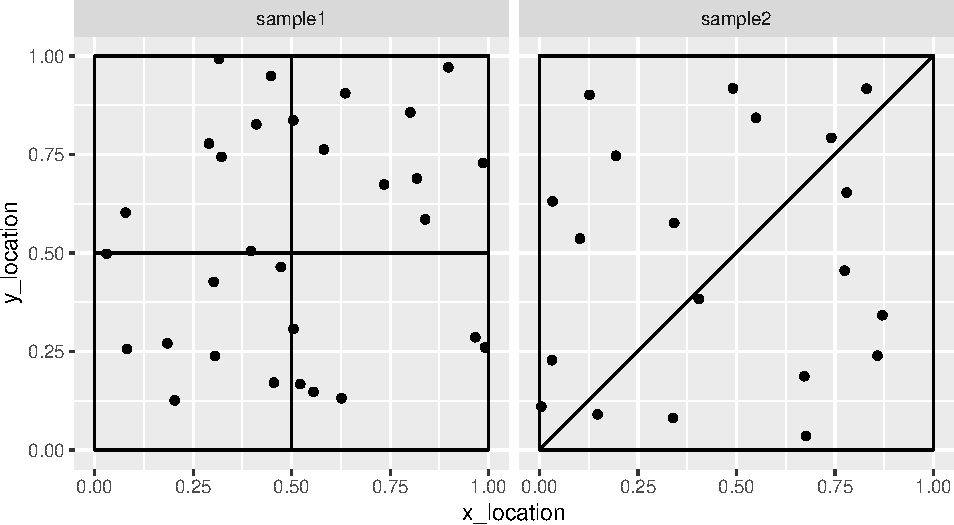
\includegraphics{bioconductor_vignette_files/figure-latex/unnamed-chunk-17-1.pdf}

The idea now is to go from a MoleculeExperiment object to a
SpatialExperiment object.

\begin{Shaded}
\begin{Highlighting}[]
\CommentTok{\#countMolecules()}
\end{Highlighting}
\end{Shaded}

\hypertarget{future-developments}{%
\section{Future developments}\label{future-developments}}

\begin{itemize}
\tightlist
\item
  SpatialUtils
\item
  one plot to show usefulness of @molecules slot
\item
  instructions on how to use readMolecules() for up-and-coming
  molecule-based ST technologies.
\end{itemize}

\hypertarget{sessioninfo}{%
\section{sessionInfo()}\label{sessioninfo}}

\begin{Shaded}
\begin{Highlighting}[]
\KeywordTok{sessionInfo}\NormalTok{()}
\end{Highlighting}
\end{Shaded}

\begin{verbatim}
## R version 4.2.1 (2022-06-23)
## Platform: x86_64-pc-linux-gnu (64-bit)
## Running under: Debian GNU/Linux 11 (bullseye)
## 
## Matrix products: default
## BLAS:   /usr/lib/x86_64-linux-gnu/openblas-pthread/libblas.so.3
## LAPACK: /usr/lib/x86_64-linux-gnu/openblas-pthread/libopenblasp-r0.3.13.so
## 
## locale:
##  [1] LC_CTYPE=C.UTF-8       LC_NUMERIC=C           LC_TIME=C.UTF-8       
##  [4] LC_COLLATE=C.UTF-8     LC_MONETARY=C.UTF-8    LC_MESSAGES=C.UTF-8   
##  [7] LC_PAPER=C.UTF-8       LC_NAME=C              LC_ADDRESS=C          
## [10] LC_TELEPHONE=C         LC_MEASUREMENT=C.UTF-8 LC_IDENTIFICATION=C   
## 
## attached base packages:
## [1] stats     graphics  grDevices utils     datasets  methods   base     
## 
## other attached packages:
## [1] ggplot2_3.4.1           SpatialUtils_0.0.0.9000 devtools_2.4.5         
## [4] usethis_2.1.6          
## 
## loaded via a namespace (and not attached):
##  [1] tidyselect_1.2.0  xfun_0.36         remotes_2.4.2     purrr_1.0.0      
##  [5] colorspace_2.1-0  vctrs_0.5.2       generics_0.1.3    miniUI_0.1.1.1   
##  [9] htmltools_0.5.4   yaml_2.3.7        utf8_1.2.3        rlang_1.0.6      
## [13] pkgbuild_1.4.0    later_1.3.0       urlchecker_1.0.1  pillar_1.9.0     
## [17] glue_1.6.2        withr_2.5.0       bit64_4.0.5       sessioninfo_1.2.2
## [21] lifecycle_1.0.3   stringr_1.5.0     munsell_0.5.0     gtable_0.3.1     
## [25] htmlwidgets_1.6.2 memoise_2.0.1     evaluate_0.20     labeling_0.4.2   
## [29] knitr_1.42        callr_3.7.3       fastmap_1.1.1     httpuv_1.6.8     
## [33] ps_1.7.3          fansi_1.0.4       highr_0.10        Rcpp_1.0.10      
## [37] xtable_1.8-4      scales_1.2.1      promises_1.2.0.1  cachem_1.0.7     
## [41] desc_1.4.2        pkgload_1.3.2     farver_2.1.1      bit_4.0.5        
## [45] mime_0.12         fs_1.6.1          digest_0.6.31     stringi_1.7.8    
## [49] processx_3.8.0    dplyr_1.1.0       shiny_1.7.4       rprojroot_2.0.3  
## [53] grid_4.2.1        cli_3.6.1         tools_4.2.1       magrittr_2.0.3   
## [57] tibble_3.2.0      profvis_0.3.7     crayon_1.5.2      pkgconfig_2.0.3  
## [61] ellipsis_0.3.2    data.table_1.14.4 prettyunits_1.1.1 rmarkdown_2.21   
## [65] rstudioapi_0.14   R6_2.5.1          compiler_4.2.1
\end{verbatim}

\end{document}
